% This file was created by tikzplotlib v0.9.5.
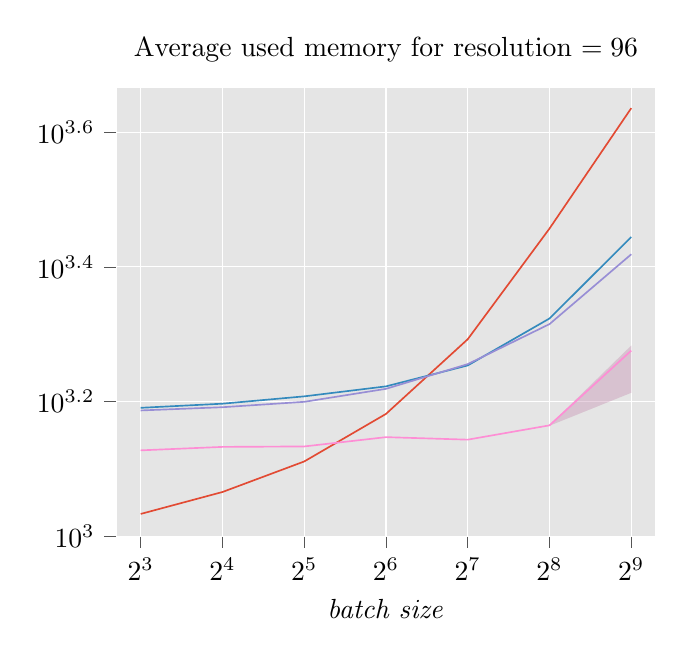
\begin{tikzpicture}

\definecolor{color0}{rgb}{0.886274509803922,0.290196078431373,0.2}
\definecolor{color1}{rgb}{0.203921568627451,0.541176470588235,0.741176470588235}
\definecolor{color2}{rgb}{0.596078431372549,0.556862745098039,0.835294117647059}
\definecolor{color3}{rgb}{0.984313725490196,0.756862745098039,0.368627450980392}
\definecolor{torchscript}{rgb}{0.996078431372549,0.556862745098039,0.835294117647059}

\begin{axis}[
axis background/.style={fill=white!89.8039215686275!black},
axis line style={white},
%legend cell align={left},
%legend style={fill opacity=0.8, draw opacity=1, text opacity=1, at={(0.03,0.97)}, anchor=north west, draw=white!80!black, fill=white!89.8039215686275!black},
log basis y={10},
tick align=outside,
tick pos=left,
title={Average used memory for resolution $=96$},
x grid style={white},
xlabel={\textit{batch size}},
xmajorgrids,
xmin=2.7, xmax=9.3,
xtick style={color=white!33.3333333333333!black},
y grid style={white},
%ylabel={memory (mb)},
ymajorgrids,
ymin=1000, ymax=4631.40123788891,
ymode=log,
ytick style={color=white!33.3333333333333!black},
xticklabels={$2^3$, $2^4$, $2^5$, $2^6$, $2^7$, $2^8$, $2^9$},
xtick={3,...,9},
]
\path [fill=color0, fill opacity=0.2, very thin]
(axis cs:3,1079)
--(axis cs:3,1079)
--(axis cs:4,1163)
--(axis cs:5,1291)
--(axis cs:6,1519)
--(axis cs:7,1961)
--(axis cs:8,2863)
--(axis cs:9,4321)
--(axis cs:9,4321)
--(axis cs:9,4321)
--(axis cs:8,2863)
--(axis cs:7,1961)
--(axis cs:6,1519)
--(axis cs:5,1291)
--(axis cs:4,1163)
--(axis cs:3,1079)
--cycle;

\path [fill=color1, fill opacity=0.2, very thin]
(axis cs:3,1551)
--(axis cs:3,1551)
--(axis cs:4,1573)
--(axis cs:5,1613)
--(axis cs:6,1669)
--(axis cs:7,1793)
--(axis cs:8,2105)
--(axis cs:9,2781)
--(axis cs:9,2781)
--(axis cs:9,2781)
--(axis cs:8,2105)
--(axis cs:7,1793)
--(axis cs:6,1669)
--(axis cs:5,1613)
--(axis cs:4,1573)
--(axis cs:3,1551)
--cycle;

\path [fill=color2, fill opacity=0.2, very thin]
(axis cs:3,1537)
--(axis cs:3,1537)
--(axis cs:4,1553)
--(axis cs:5,1583)
--(axis cs:6,1655)
--(axis cs:7,1801)
--(axis cs:8,2065)
--(axis cs:9,2621)
--(axis cs:9,2623)
--(axis cs:9,2623)
--(axis cs:8,2065)
--(axis cs:7,1801)
--(axis cs:6,1655)
--(axis cs:5,1583)
--(axis cs:4,1555)
--(axis cs:3,1537)
--cycle;

\path [fill=white!46.6666666666667!black, fill opacity=0.2, very thin]
(axis cs:3,1341)
--(axis cs:3,1341)
--(axis cs:4,1357)
--(axis cs:5,1359)
--(axis cs:6,1403)
--(axis cs:7,1391)
--(axis cs:8,1459.14)
--(axis cs:9,1633)
--(axis cs:9,1919)
--(axis cs:9,1919)
--(axis cs:8,1461)
--(axis cs:7,1391)
--(axis cs:6,1403)
--(axis cs:5,1359)
--(axis cs:4,1357)
--(axis cs:3,1341)
--cycle;

\path [fill=torchscript, fill opacity=0.2, very thin]
(axis cs:3,1341)
--(axis cs:3,1341)
--(axis cs:4,1357)
--(axis cs:5,1359)
--(axis cs:6,1403)
--(axis cs:7,1391)
--(axis cs:8,1459.14)
--(axis cs:9,1633)
--(axis cs:9,1919)
--(axis cs:9,1919)
--(axis cs:8,1461)
--(axis cs:7,1391)
--(axis cs:6,1403)
--(axis cs:5,1359)
--(axis cs:4,1357)
--(axis cs:3,1341)
--cycle;

\addplot [semithick, color0]
table {%
3 1079
4 1162.99987792969
5 1290.99975585938
6 1518.99963378906
7 1961.00012207031
8 2863.00073242188
9 4321.0009765625
};
%\addlegendentry{cudnn}
\addplot [semithick, color1]
table {%
3 1551.00012207031
4 1573
5 1613.00024414062
6 1669.00048828125
7 1793.00012207031
8 2105.00048828125
9 2781
};
%\addlegendentry{libtorch}
\addplot [semithick, color2]
table {%
3 1537
4 1554.19982910156
5 1583.00036621094
6 1654.99975585938
7 1800.99975585938
8 2064.99951171875
9 2621.69946289062
};
%\addlegendentry{pytorch}
\addplot [semithick, torchscript]
table {%
3 1341
4 1356.99987792969
5 1359.00012207031
6 1403.00036621094
7 1391.00036621094
8 1460.81384277344
9 1886.31420898438
};
%\addlegendentry{torchscript}
\end{axis}

\end{tikzpicture}
